\documentclass[11pt,]{article}
\usepackage{lmodern}
\usepackage{amssymb,amsmath}
\usepackage{ifxetex,ifluatex}
\usepackage{fixltx2e} % provides \textsubscript
\ifnum 0\ifxetex 1\fi\ifluatex 1\fi=0 % if pdftex
  \usepackage[T1]{fontenc}
  \usepackage[utf8]{inputenc}
\else % if luatex or xelatex
  \ifxetex
    \usepackage{mathspec}
  \else
    \usepackage{fontspec}
  \fi
  \defaultfontfeatures{Ligatures=TeX,Scale=MatchLowercase}
\fi
% use upquote if available, for straight quotes in verbatim environments
\IfFileExists{upquote.sty}{\usepackage{upquote}}{}
% use microtype if available
\IfFileExists{microtype.sty}{%
\usepackage{microtype}
\UseMicrotypeSet[protrusion]{basicmath} % disable protrusion for tt fonts
}{}
\usepackage[margin=1in]{geometry}
\usepackage{hyperref}
\hypersetup{unicode=true,
            pdftitle={Speakers of diverse languages structure their utterances for efficient communication},
            pdfauthor={Josef Klafka and Daniel Yurovsky},
            pdfborder={0 0 0},
            breaklinks=true}
\urlstyle{same}  % don't use monospace font for urls
\usepackage{longtable,booktabs}
\usepackage{graphicx,grffile}
\makeatletter
\def\maxwidth{\ifdim\Gin@nat@width>\linewidth\linewidth\else\Gin@nat@width\fi}
\def\maxheight{\ifdim\Gin@nat@height>\textheight\textheight\else\Gin@nat@height\fi}
\makeatother
% Scale images if necessary, so that they will not overflow the page
% margins by default, and it is still possible to overwrite the defaults
% using explicit options in \includegraphics[width, height, ...]{}
\setkeys{Gin}{width=\maxwidth,height=\maxheight,keepaspectratio}
\setlength{\emergencystretch}{3em}  % prevent overfull lines
\providecommand{\tightlist}{%
  \setlength{\itemsep}{0pt}\setlength{\parskip}{0pt}}
\setcounter{secnumdepth}{5}
% Redefines (sub)paragraphs to behave more like sections
\ifx\paragraph\undefined\else
\let\oldparagraph\paragraph
\renewcommand{\paragraph}[1]{\oldparagraph{#1}\mbox{}}
\fi
\ifx\subparagraph\undefined\else
\let\oldsubparagraph\subparagraph
\renewcommand{\subparagraph}[1]{\oldsubparagraph{#1}\mbox{}}
\fi

%%% Use protect on footnotes to avoid problems with footnotes in titles
\let\rmarkdownfootnote\footnote%
\def\footnote{\protect\rmarkdownfootnote}

%%% Change title format to be more compact
\usepackage{titling}

% Create subtitle command for use in maketitle
\providecommand{\subtitle}[1]{
  \posttitle{
    \begin{center}\large#1\end{center}
    }
}

\setlength{\droptitle}{-2em}

  \title{Speakers of diverse languages structure their utterances for efficient communication}
    \pretitle{\vspace{\droptitle}\centering\huge}
  \posttitle{\par}
    \author{Josef Klafka and Daniel Yurovsky}
    \preauthor{\centering\large\emph}
  \postauthor{\par}
      \predate{\centering\large\emph}
  \postdate{\par}
    \date{2019-09-09}

\usepackage{setspace}

\doublespacing

\begin{document}
\maketitle

\hypertarget{abstract}{%
\section{Abstract}\label{abstract}}

Language can be thought of as a code: speakers encode their thoughts into a sequence of linguistic signals, namely an utterance, which listeners then must decode in order to recover the intended message. How do speakers structure their utterances so that communication is successful? Using tools from information theory and sentence processing, we find that speakers must structure the information in their utterances according to the grammatical, morphological and lexical constraints of their language, which vary greatly from language to language. This information structure characterizes language from children's first utterances to large-scale knowledge base entries. Once listeners have access to linguistic context within an utterance, then they can decode the rest of that utterance at a constant and optimal rate.

\hypertarget{introduction}{%
\section{Introduction}\label{introduction}}

We use language to communicate information. Although we often need to say things we have never said before, we are easily and efficiently able to produce novel utterances with minimal prior planning. Our listeners incrementally process our utterances, and predict which words will come next within fractions of a second of hearing the beginning of the word (for evidence see e.g.~Kutas \& Federmeier, 2010). Encoding new and unpredictable information into our utterances surprises our listeners, and presents problems for communication. Listeners struggle to decode unpredictable words and may have difficulty decoding the following words as well. Efficient and effective communication relies on interlocutors being able to process novel information in without being surprised by new information in unpredictable words. On the other hand, to make best use of the capacity of the communication channel, speakers should encode as much information as possible into each word they say.

Due to their differences in distributional frequency, words vary in how much information-theoretic content they contain (Shannon, 1948). This information content plays an important role in determining the shape of words and speech. Frequency is a meaningful predictor of word length: the more common the word, the shorter the word tends to be as speakers minimize effort in the amount of information they encode in speech (Zipf, 1949). Over and above frequency, contextual information content predicts word length (Piantadosi, Tily \& Gibson, 2011). Speakers tend to smooth out their information to a more uniform rate within utterances that allows for easier decoding on the listener side (Jaeger \& Levy, 2007). Across utterances, context allows speakers to produce more informative and surprising sentences later in communication. The later a sentence occurs in a paragraph, the the informative it is and the more unusual and surprising words it contains (Genzel \& Charniak, 2002). From the level of individual words to sentences in paragraphs, information content shapes and is shaped by the context it appears in.

However, a gap exists in the literature for examining how frequency and context determine the information content in utterances. We do not speak only in phrases or paragraphs, but conversationally we communicate in utterances, either on their own or banded together. Writers use sentences to communicate thoughts, often on their own instead in paragraphs with other sentences. Cross-linguistically, the average rate of information speakers transfer in a syllable differs (Aylett \& Turk, 2004). Languages possess very different grammatical and morphological structures--the same thought can be encoded in at least as many ways as there are different languages. How do the different structures seen in different languages, with different rates of information encoding, affect how speakers structure information in production?

Yu, Cong, Liang, \& Liu (2016) proposed a novel method for quantifying the amount of information typically found at each part of English utterances. The Yu et al work examined written sentences from the British National Corpus. Treating each word position by itself, Yu et al.~calculated the Shannon entropy (a measure of uncertainty) over the words of each position, producing an estimate for the amount of uncertainty reduced once the listener hears the words used in a given position, related to the Shannon concept of information as a reduction in uncertainty (Shannon, 1948). Yu et al.~found a distinctive three-step shape to the distribution of information in the British National Corpus.

In this paper, we expand on this body of prior work in a number of novel ways. We replicate Yu et al's results with a different metric, one intimately tied to incremental word processing. We find the same distribution of information based on word frequency in English adult speech as in English adult writing, as well as in English child speech. We expand the study of information density to the largest set of languages yet considered, and incorporate contextual and typological information. We find that each language has a characteristic, robust distribution of information predictable from its morphology, phonology and syntax, and tied to the language's genealogy. Speakers of a language will tend to distribute information according to that language's distribution of information in their utterances. As soon as a child can form multi-word utterances in a given language, they will produce utterances obeying the characteristic distribution of information in a given language. We also apply a contextual version of the same metric, and find that in communication, listeners are able to decode information from the utterances they hear at a constant rate, regardless of language, past the first couple of words.

\hypertarget{methods}{%
\section{Methods}\label{methods}}

Shannon (1948) defined information as ``the reduction in uncertainty about one variable given that the value of another variable is known''. We use a metric proposed by Shannon and applied by Levy (2008): lexical surprisal, which defines the information in word based on the ratio of possible continuations of the sentence after to before the word is seen. Equivalently, we can compute surprisal with the predictability of the word, as in the formula below. The surprisal of a word is inversely proportional to the predictability of a word, such that less common and less predictable words carry more information.

\[surprisal(word) = -log P(word)\]

The surprisal of a word is also correlated with the processing cost of a word, with evidence from eye-tracking (Smith \& Levy, 2013) and ERP (Frank, Otten, Galli, \& Vigliocco, 2015) studies, among other sources. Considered without context, the surprisal of an individual word is inversely proportional to the frequency of that word, so that the less often a person has seen a word, the more information that word holds. For example, ``flower'' has less information than ``azalea'' because ``flower'' is much more common than ``azalea''. Though the two words have the same length in number of letters, it's more difficult to process ``azalea'' when reading it here than when reading ``flower''. Frequency is intimately tied information content in words, with much of the differences between words frequencies being explained by information content cross-linguistically (Piantadosi, Tily, \& Gibson, 2011).

However, when reading or listening, people don't just consider each word as an isolated linguistic signal. Instead, listeners use the words they have already heard to predict and decode the word they are currently processing. Following this incremental processing paradigm, we can also condition the surprisal of a word in its context. In the formula below, widenotes the word currently being read or heard, while wi-1denotes the first word before the current word, wi-2denotes the second word before the current word, and so on.

\[surprisal(w_i|w_{i-1}w_{i-2}...) = -log P(w_i|w_{i-1}w_{i-2}...)\]
\[= -log \frac{P(w_i,w_{i-1}w_{i-2},...)}{P(w_{i-1}w_{i-2}...)}\]

When we use a word or two of context in our surprisal calculations, then the set of reasonable final items in our ngrams is greatly restricted. ``Flower'' may contain less information than ``azalea'' when we consider the words independently of their context, but with context this can be reversed. Flower appears in a variety of contexts, and so the information content of a word like ``flower'' in a particular context may be higher than ``azalea''. If you only have azaleas in your garden, then hearing someone say ``in that garden, look at the flowers'' may be higher surprisal for you: you expect them to say ``azalea''. This prediction does not need many words before to work out, for example in ``I take my coffee with cream and sugar''. When you hear ``cream and'', you automatically predict ``sugar'' or maybe ``honey'', but there are few possible continuations with even those two words. Hearing ``I'' restricts the next word to a verb, or possibly an adverb, and since you have just heard the speaker refer to themselves in the first person singular, your set of possible completions is significantly restricted.

To find the distribution of information within a corpus, we calculate the surprisal or contextual surprisal for each unique word or sequence of words within the corpus. We take all utterances of a given length, and for each word position in utterances of that length, we compute the average of the surprisals for all of the non-unique words that occur in that position, conditioned or not conditioned on context. By computing these averages for each word position in an utterance, we compute a low-dimensional approximation to the average distribution of information in the corpus. With the surprisal metric, we base the information contained in each word on how often the word is encountered in its context in the corpus. As long as the corpus is representative of the language or population we study, then the distribution of information is approximated for that language or population as a whole.

The frequency-based surprisal metric gives us an idea of when in their utterances speakers say frequent i.e.~independently information-rich words. The context-based surprisal metric show us how speakers tend to distribute the information in utterances relative to real-time processing in communication. We expect a priori that our frequency-based surprisal curve will be flat. No one part of the sentence will on average have words that are more frequent than another across utterance lengths. Similarly, we expect that there will be a small smoothing effect for our contextual surprisal metric.

\hypertarget{written-and-spoken-english-have-the-same-information-distribution}{%
\section{Written and Spoken English have the same information distribution}\label{written-and-spoken-english-have-the-same-information-distribution}}

We first turn to working with written English in the British National Corpus (BNC). The BNC is a collection of spoken and written records (90\% written) from the turn of the century, intended to be a representative sample of British English. Using their word entropy metric without context, Yu et al.~found a distinctive three-step distribution for information in written English sentences in the corpus. The first word tended to contain little information. While the middle words of sentences each had more information than the first word, information was flat and non-increasing across the middle of sentences. The final word, they found, contained the most information out of any in the sentence, with a noticeable spike in information. They found the same distribution across sentence lengths, from sentences with 15 words to sentences with 45 words.

We first replicate the Yu et al. (2016) result using the surprisal metric in place of the entropy metric. We use the frequency-based or ``contextless'' surprisal metric, which determines the average distribution of information based on word frequencies in a corpus. A priori we expect that the frequency-based metric will produce a flat distribution of information across word positions in the BNC.

See in the figure below a qualitative comparison of the information trajectory they found and the information trajectory we found. It is easily observable that the two information trajectories are identical, and we have found the same distribution of information in the BNC as Yu et al did. The first words in written English sentences tend to contain little information, while the final words tend to contain a great deal of information.

Comparison between the unigram entropy and surprisal BNC results plot

However, this only characterizes written English sentences. If this information distribution is characteristic more generally of English, then we will find the same distribution for spoken English. We use the Switchboard corpus of spoken English telephone conversations between adults to compute the distribution of information across spoken utterances in English. The sentences in the BNC, compared to the conversations in Switchboard, feature much longer sentences with larger vocabularies and more complex sentence structures. We split the conversations in Switchboard not by sentences, as in the BNC, but by turns.

For Switchboard we find the same information trajectory as we did for the BNC, and we find the same distribution of information regardless of utterance length. The longer the utterance, the more pronounced the information distribution shape becomes. A qualitative comparison of the two trajectories is below.

We have found a unique average distribution of information that appears to characterize the English language as a whole, regardless of medium (spoken or written) or utterance length. This distribution indicates that in English, the words we speak or write at the beginnings of utterances has little information, while the words we speak or write at the ends of utterances has a lot of information. The words in the middle of utterances have a middling amount of information, without the increasing trend in information from word to word that we might expect from (Genzel \& Charniak, 2002).

What about context? So far we've only discussed the unigram (``contextless'') surprisal metric, considering words on their own without any explicit incorporation of prior context. As previously discussed, listeners decode information and process what they hear incrementally, using prior heard words to ease the comprehension process. We now include one word of context (bigrams) and then two words of context (trigrams). We observe a flattening effect of context across both modalities and all speaker populations. After the first word or two, where the listener does not have access to prior context, then they decode information at a flat and more or less uniform rate.

Speakers produce information at a more or less constant rate, avoiding peaks or troughs in their information distribution, except at the beginnings of utterances, where listeners may not have any context to predict what the speaker is going to say. Speakers of English tend towards a characteristic and uneven distribution of word information based on frequencies within their utterances. Their interlocutors, however, once they have a word or two of context, decode information at a more or less constant and optimal rate.

\hypertarget{english-cds-and-child-speech}{%
\section{English CDS and child speech}\label{english-cds-and-child-speech}}

We found that English speakers and writers used the same robust and distinctive distribution of information within each utterance, regardless of the number of words in their utterances. To determine if this distribution truly characterizes all speakers of the English language as a whole, we wanted to examine speech from English-speaking children who are producing their very first multi-word utterances. We hypothesize the three-step distribution of information we found for English will characterize child speech and child-directed speech.

We use the Providence corpus from CHILDES (Evans \& Demuth, 2012; MacWhinney, 2000), which consists of about 650000 utterances from parent-child conversations for six monolingual English-speaking children talking with the parents. The child age range was between 11 months and 4 years. Sessions recorded in the home. Parents said a majority of the utterances, but children take up an increasing share of the conversation as they grow older and are actually able to speak full utterances. The utterances in the Providence corpus are on average significantly shorter than those in the BNC and Switchboard; over 90\% of the utterances in the Providence corpus are at most 10 words long, with the median at around 6 words. Similar to our treatment of the Switchboard corpus, we split the Providence corpus up by conversational turns and separate utterances.

We observe the same distinctive distribution of information for parents and children in the Providence corpus as we did for adults in the BNC and Switchboard. The distribution of information we found at the level of individual words in English, therefore, characterizes the English language as a whole and not only adult utterances, not only written utterances.

\begin{figure}
\centering
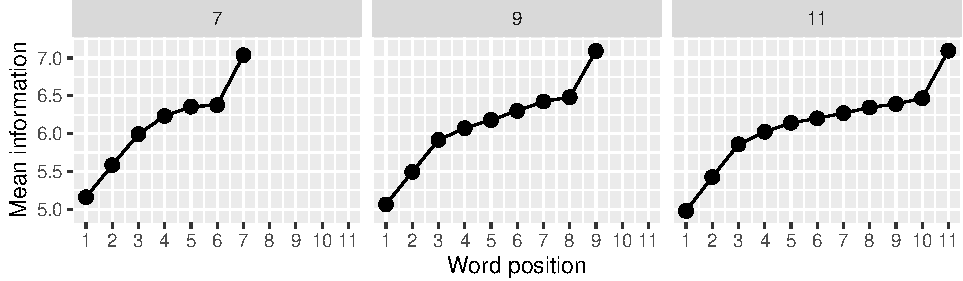
\includegraphics{paper_files/figure-latex/unnamed-chunk-1-1.pdf}
\caption{\label{fig:unnamed-chunk-1}Providence frequency-based information curves}
\end{figure}

What about context in the Providence corpus? When incorporating one or two words of predictive context, we observe the same trend as in the Switchboard and BNC corpora. Beyond the first couple of words, once your interlocutor has enough context to predict with some accuracy what you will say next, then you decode information from their speech stream at a constant and optimal rate. This applies to parents and children speaking to one another, as well as adults speaking and writing to one another.

\begin{figure}
\centering
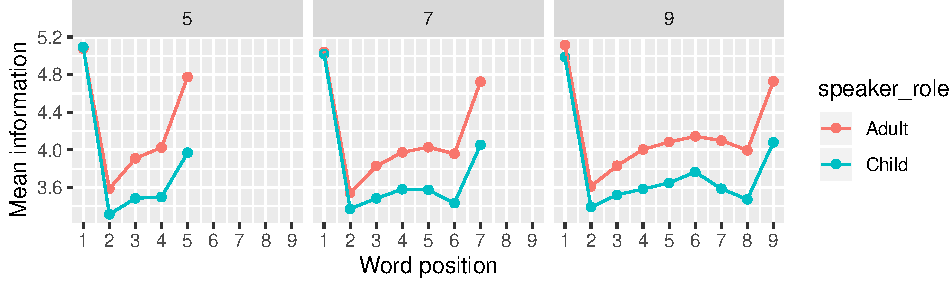
\includegraphics{paper_files/figure-latex/unnamed-chunk-2-1.pdf}
\caption{\label{fig:unnamed-chunk-2}Providence bigram context-based information curves}
\end{figure}

\begin{figure}
\centering
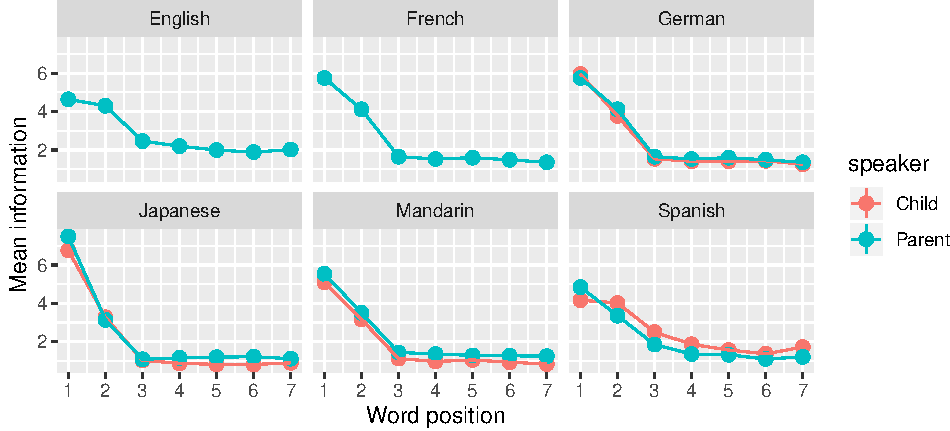
\includegraphics{paper_files/figure-latex/unnamed-chunk-3-1.pdf}
\caption{\label{fig:unnamed-chunk-3}Providence trigram context-based information curves}
\end{figure}

\hypertarget{child-speech-and-cds-across-languages}{%
\section{Child speech and CDS across languages}\label{child-speech-and-cds-across-languages}}

So far, we have only looked at the distribution of information in words in English, both with and without context. We have examined child speech, child-directed speech and adult-directed speech, as well as writing samples selected to be representative of British English as a whole. But this only captures the picture for English.

We now turn to a small number of typologically diverse languages, and conduct the same analysis, using a monolingual adult-child speech corpora from CHILDES (MacWhinney, 2000) to compare the results from these languages directly to our results from the English Providence corpus. We use corpora for Spanish, German, French, Mandarin and Japanese. Similarly to the English Providence corpus, all of the following corpora consist mainly of shorter utterances: most utterances in the corpora are under 10 words long. For Spanish, we use the corpus of conversations between primary school-aged children between 6 and 9 years old and the researchers, in which the children were asked to recite stories in their native Spanish (Shiro, 1997). The students came from working class public schools and upper class private schools. For German, we use the Wagner corpus (Wagner, 1985). This corpus consists of a collection of mini-corpora collected from socio-economically diverse families, with children aged from 1;0 to 14;0, mainly on the younger end of that range. The corpus mainly consists of parent-child conversations between the children and their primary caregivers. For French, we use the Palasis corpus (Palasis, 2009), a longitudinal study of children between the ages of 2;5 and 4;0 from the same kindergarten class. The conversations in this corpus take place between the children and other children in the same class, and between the children and the investigator. For Mandarin Chinese, we use the Zhou corpus of dinner conversations from the Shanghai area (Li \& Zhou, 2015). The children in this corpus are 5 or 6 years old, and half come from working class families (the other half from upper class families). For Japanese, we use the Okayama corpus (Okayama, 1973). This corpus consists of conversations between children between the ages of 2;2 and 4;2 and their mothers.

We observe a distinct and characteristic frequency-based information trajectory emerge for each language, robust across each utterance length within each language. We see the same distribution of information for both parents and children in each language, with the child's curve normally below the parent's curve, likely due to the parent speaking a larger share of the utterances in the corpus and using a larger vocabulary than the child. We see the opposite amplitude trend in the Shiro corpus, where the children speak more than the adult investigators as the children are the ones telling the stories. We include the frequency-based information curve from the Providence corpus for comparison.

\begin{figure}
\centering
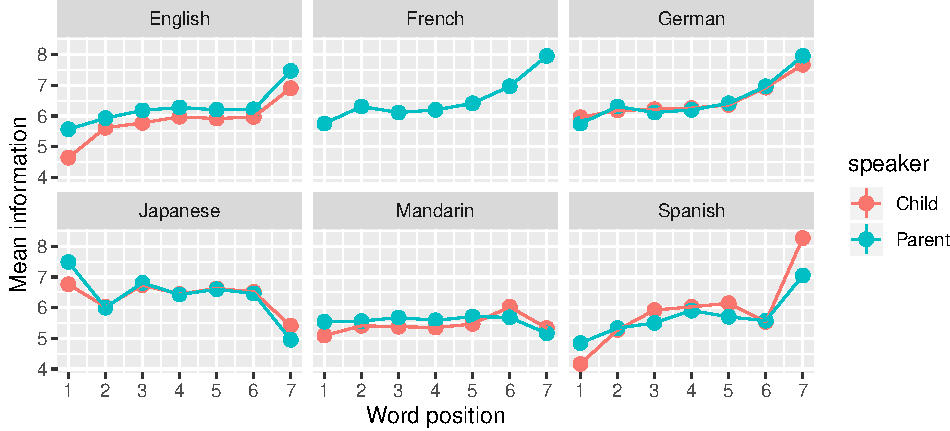
\includegraphics{paper_files/figure-latex/unnamed-chunk-4-1.pdf}
\caption{\label{fig:unnamed-chunk-4}CHILDES frequency-based information curves}
\end{figure}

English, Spanish, French and German feature similar information curves shapes, with slight variations. The German information curve features lower information for longer towards the beginnings of utterances, possibly due to the grammatical restriction that the second word in German utterances must be a verb (V2). Spanish features a larger spike in the amount of information in the final words of utterances. For Japanese and Mandarin, we observe completely different unigram information curve trajectories. The Japanese unigram information curve trajectory begins high and finishes low, the mirror image of the European language information curves. The Mandarin curve begins low and finishes low, but features high information in the middle of utterances. We hypothesize this may be due to both Japanese and Mandarin speakers typically ending their utterances with particles, which contain very little information on their own. The penultimate noun with the speakers pair the particles are where the information lies.

For the bigram and trigram information curves, we see the same contextual smoothing effect as for all the corpora we worked with in English. While the unigram information curves may depend based on the language, the contextual information curves show the same trajectory cross-linguistically. Using ngrams with n higher than 3 is difficult for parent-child speech corpora because the utterances are so short on average (less than 10 words). We hypothesize that the unigram information curves may vary based on the genealogy and typology of the languages in question, but this does not extend to the trigram information curves in particular. We shall show evidence that this is true in the rest of the paper.

\begin{figure}
\centering
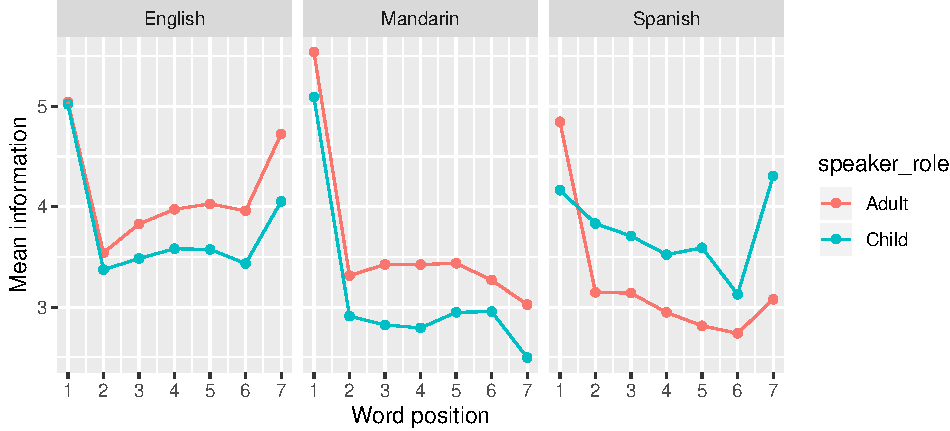
\includegraphics{paper_files/figure-latex/unnamed-chunk-5-1.pdf}
\caption{\label{fig:unnamed-chunk-5}CHILDES bigram context-based information curves}
\end{figure}

\begin{figure}
\centering
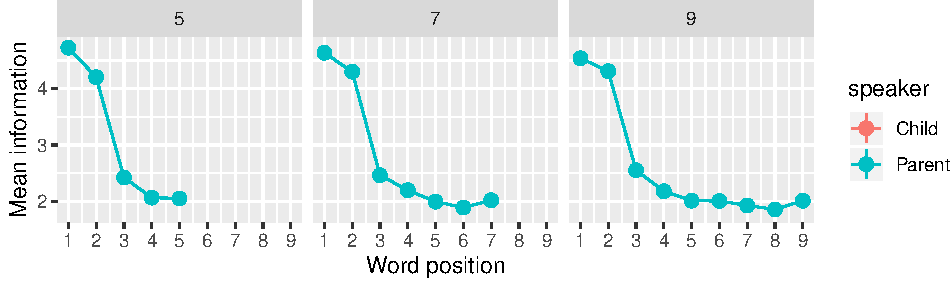
\includegraphics{paper_files/figure-latex/unnamed-chunk-6-1.pdf}
\caption{\label{fig:unnamed-chunk-6}CHILDES trigram context-based information curves}
\end{figure}

\hypertarget{language-structure-and-large-scale-data-analysis-methods-and-preprocessing}{%
\section{Language structure and large-scale data analysis: methods and preprocessing}\label{language-structure-and-large-scale-data-analysis-methods-and-preprocessing}}

To make a claim about language as a whole and languages on a larger scale, we needed to use larger corpora and a much larger number of languages. We pulled corpora for 159 diverse languages from Wikipedia {[}Citation{]}, each of which had at least 10000 articles. We split each article up into sentences; the variance in sentence lengths for Wikipedia was significantly larger than for the CHILDES corpora we used in the previous section. Most sentences in Wikipedia contained between 10 and 30 words, unlike the CHILDES corpora which mainly contained utterances with under 10 words. We excluded the small fraction of utterances with more than 50 words as uncharacteristic of English speech.

How to analyze more than 40 different surprisal curves for each language, adding up to several thousand surprisal curves total? We used two different strategies, which yielded identical results upon analysis. Each strategy gave us a five-dimensional vector space embedding for each language in a Wikipedia ``slope space''. For the first strategy, we split each sentence length by number of words into fifths, and computed surprisal values for the closest word position to each quintile. We then computed the slopes between the surprisal values at neighboring quintiles, yielding five slope values for each curve. For the second strategy, we split each sentence length by number of words into sections based on those areas of the surprisal curves that had seemed most important before: between the first and second word; between the second and third word; between the third word and third-to-last word; between the third-to-last word and the second to last word; and between the second-to-last word and the last word. We then similarly computed surprisal values at each of these positions, and similarly computed slopes between the surprisal values at each position, giving us another five slope values for each language summarizing the surprisal curves. Illustrations of these two strategies are below.

Illustration of the regions we target with each of the two slope treatments below.

We computed unigram, bigram and trigram values for each language. All of this data, along with the scripts used for the analysis, are available on GitHub. We ran this code on the RCC at the University of Chicago; it took X amount of time and used up Y amount of carbon to run.

To more rigorously described the differences between languages, we used data from the World Atlas of Language Structures (WALS; Dryer \& Haspelmath eds., 2013). WALS has data for 144 typological features in 2569 languages around the world. These features describe aspects of morphology, syntax, phonology, etymology and semantics--in short the features describe the structures in each language. As WALS is a compiled database from dozens of papers from different authors, most of the features and languages are fairly sparse. Even limiting ourselves to the 159 language corpora we pulled from Wikipedia and 122 features from WALS, there are nearly 20000 individual possible feature values, fewer than half of which were already inputted for those languages in the WALS database.

We used the Multiple Imputation Multiple Correspondence Analysis algorithm (MIMCA; Citation) to fill in the missing data using statistical imputation. MIMCA essentially uses mean imputation to begin with the missing values, then performs repeatedly performs principle components analysis on and reconstructs the contingency table formed from observations in categorical variables. By the end of this we had unigram, bigram and trigram surprisal curves for the 159 language corpora pulled from Wikipedia, along with 122 typological features for each language.

However, the WALS features describe specific structural differences between languages, while our surprisal metric is lexical. To target lexical differences between languages, we computed the average normalized Levenshtein distance (LDN; Holman et al, 2008) over the 40 item Swadesh list (1955), retrieved from the ASJP database (Wichmann, Holman \& Brown, 2018). The Swadesh list is designed to include near-universal words that target basic cognitive concepts, and are useful in determining the genealogical similarities and differences between languages. The results of classifying languages using the Swadesh list and LDN are correlated with those using WALS features, but the Swadesh list and LDN do not suffer from the same sparsity problem as WALS (Holman et al, 2008).

\hypertarget{language-structures-and-large-scale-data-analysis-results}{%
\section{Language structures and large-scale data analysis: results}\label{language-structures-and-large-scale-data-analysis-results}}

We ran a hierarchical clustering algorithm on the unigram information curves using the hclust package in R (hclust). We used the complete linkage algorithm for hierarchical clustering with distances between information curves in language computed using cosine distance between their embeddings in the slope space. The complete linkage algorithm at every step pairs each language or cluster of languages with its closest neighboring language or cluster. A sample from the dendrogram is shown below, and the full tree can be constructed using the code in our GitHub repository. The language family-like structure can be seen at first glance, although the dendrogram does not exactly replicate language genealogy for all 159 languages. This suggests using a first-pass quantitative method that the information curves do correspond in some measure to language families, but language families do not explain the entire story.

Dendro goes here

A sample of the trigram information curves are plotted below, and all trigram information curves for the languages we used follow the same pattern. The first few words in utterances for each language are surprising, but with even a couple words of predictive context for each word, the amount of information in each word drops off and speakers produce information at a constant, optimal rate.

Plot of some trigram surprisal curves goes here

First we examined the effects of individual typological features on the shapes of the unigram information curves. We ran logistic regressions using the lme4 package in R (lme4), checking whether the cosine distance between two languages' embeddings in the slope space played a role in determining if they had the same value for a given WALS feature. Individual WALS features do not necessarily have ordinal values. Some, such as the ``Number of Cases'' feature, are easy to quantify and order. Others are more difficult. For example, how does one order ``relative clauses appear after the nouns they modify'', ``relative clauses appear before the nouns they modify'' and ``free order of relative clauses and nouns''? We chose the identify relation to avoid deciding on the basis of individual features. We found that 100 out of the 120 features from WALS we examined was statistically significant (p \textless{} .001) in determining whether two languages had the same shape to their unigram information distributions. The results for some important features are below, and the rest of the results are in the Appendices.

Some lr results go here.

We next compared how the cosine distance between two languages related to how many WALS features they had in common. There is a small correlation with a very small R\^{}2 value between WALS features similarity and cosine similarity between two languages, but a statistically significant slope (p \textless{} .001). Essentially, for every feature two languages have in common, they have one degree more cosine similarity in the slope space. As feature values tend to be highly correlated within categories (e.g.~the word order features are highly correlated), then this translates into language having much more similar information curves if they have more WALS features in common, an intuitive result.

\begin{figure}
\centering
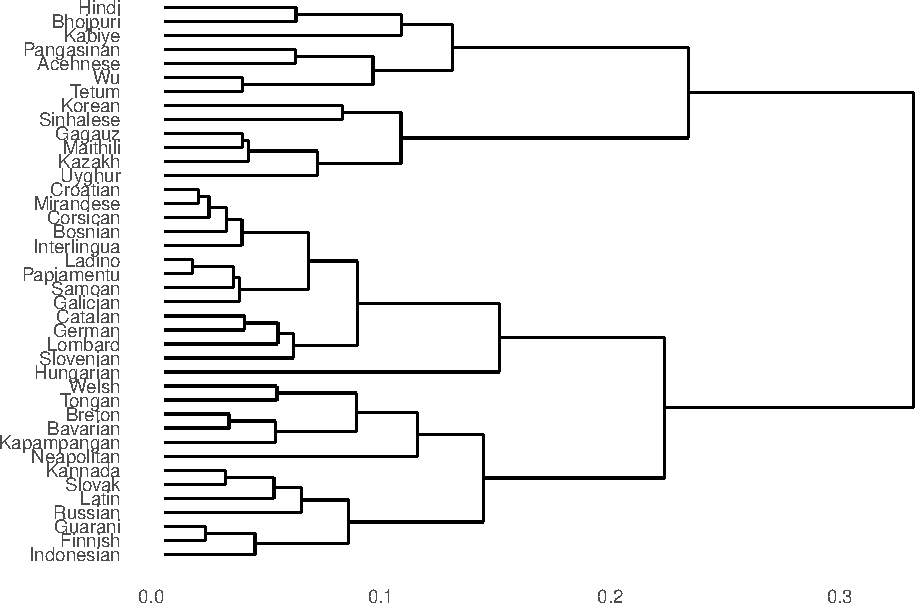
\includegraphics{paper_files/figure-latex/unnamed-chunk-7-1.pdf}
\caption{\label{fig:unnamed-chunk-7}wals features vs cosine similarity}
\end{figure}

So the more similar two languages are in terms of typological features, the more similar their unigram information curves tend to be. For lexical features, we see a stronger correlation between the similarity of two languages in terms of their average LDN and the cosine distance between their information curves.

\begin{figure}
\centering
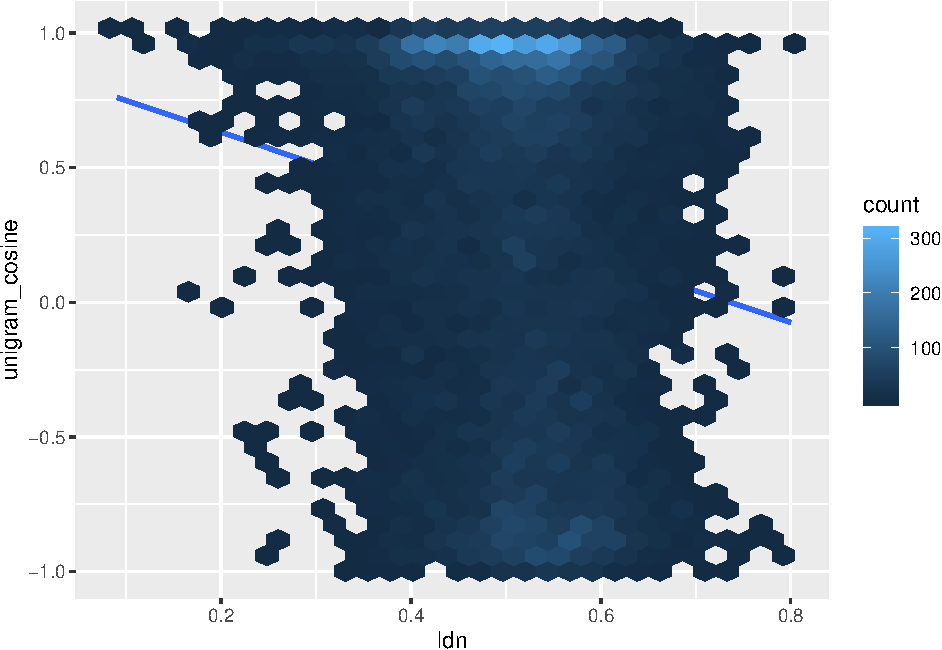
\includegraphics{paper_files/figure-latex/unnamed-chunk-8-1.pdf}
\caption{\label{fig:unnamed-chunk-8}ldn features vs cosine similarity}
\end{figure}

The shape of a language's frequency-based information curve covaries with its typological and lexical similarity to other languages.

\hypertarget{general-discussion}{%
\section{General Discussion}\label{general-discussion}}

The language we speak impacts how we encode information into our utterances, and how listeners decode our speech signals. However, despite the variety in communicative codes, all languages are characterized by predictability and a lack of suprisal in regular speech. In this paper, we developed a novel computational modeling method for examining the average information at a fine-grained level in utterances of different lengths in a variety of corpora and across a large number of languages. With only a couple of words of context for each word, cross-linguistic differences disappear and all languages are characterizes by low surprisal (low processing cost and information).

The Uniform Information Density Hypothesis (Levy \& Jaeger, 2007) provides an optimal strategy for distributing information among the words in an utterance. The hypothesis suggests that speakers tend to distribute information evenly in their utterances, close to the capacity of the communication channel. This strategy avoids peaks in information which lead to issues for the decoder, while making the best use of the communication channel possible and aiming to produce as much information as the listener can decode at every moment.

\hypertarget{references}{%
\section*{References}\label{references}}
\addcontentsline{toc}{section}{References}

\hypertarget{refs}{}
\leavevmode\hypertarget{ref-aylett2004smooth}{}%
Aylett, M., \& Turk, A. (2004). The smooth signal redundancy hypothesis: A functional explanation for relationships between redundancy, prosodic prominence, and duration in spontaneous speech. \emph{Language and Speech}, \emph{47}(1), 31--56.

\leavevmode\hypertarget{ref-evans2012individual}{}%
Evans, K. E., \& Demuth, K. (2012). Individual differences in pronoun reversal: Evidence from two longitudinal case studies. \emph{Journal of Child Language}, \emph{39}(1), 162--191.

\leavevmode\hypertarget{ref-frank2015erp}{}%
Frank, S. L., Otten, L. J., Galli, G., \& Vigliocco, G. (2015). The erp response to the amount of information conveyed by words in sentences. \emph{Brain and Language}, \emph{140}, 1--11.

\leavevmode\hypertarget{ref-genzel2002entropy}{}%
Genzel, D., \& Charniak, E. (2002). Entropy rate constancy in text. \emph{Proceedings of the 40th annual meeting of the association for computational linguistics}, 199--206.

\leavevmode\hypertarget{ref-jaeger2007speakers}{}%
Jaeger, T. F., \& Levy, R. P. (2007). Speakers optimize information density through syntactic reduction. \emph{Advances in neural information processing systems}, 849--856.

\leavevmode\hypertarget{ref-levy2008expectation}{}%
Levy, R. (2008). Expectation-based syntactic comprehension. \emph{Cognition}, \emph{106}(3), 1126--1177.

\leavevmode\hypertarget{ref-macwhinney2000childes}{}%
MacWhinney, B. (2000). \emph{The childes project: The database} (Vol. 2). Psychology Press.

\leavevmode\hypertarget{ref-piantadosi2011word}{}%
Piantadosi, S. T., Tily, H., \& Gibson, E. (2011). Word lengths are optimized for efficient communication. \emph{Proceedings of the National Academy of Sciences}, \emph{108}(9), 3526--3529.

\leavevmode\hypertarget{ref-shannon1948mathematical}{}%
Shannon, C. E. (1948). A mathematical theory of communication. \emph{Bell System Technical Journal}, \emph{27}(3), 379--423.

\leavevmode\hypertarget{ref-smith2013effect}{}%
Smith, N. J., \& Levy, R. (2013). The effect of word predictability on reading time is logarithmic. \emph{Cognition}, \emph{128}(3), 302--319.

\leavevmode\hypertarget{ref-yu2016distribution}{}%
Yu, S., Cong, J., Liang, J., \& Liu, H. (2016). The distribution of information content in english sentences. \emph{arXiv Preprint arXiv:1609.07681}.

\leavevmode\hypertarget{ref-zipf1949human}{}%
Zipf, G. K. (1949). \emph{Human behavior and the principle of least effort.}


\end{document}
